\section{Other capacitive prototypes}
\label{ch:prot_otherprot}
In collaboration with other partners from industry and different students some additional prototypes have been created that are discussed briefly in this section. 

\begin{figure}[ht]
\centering
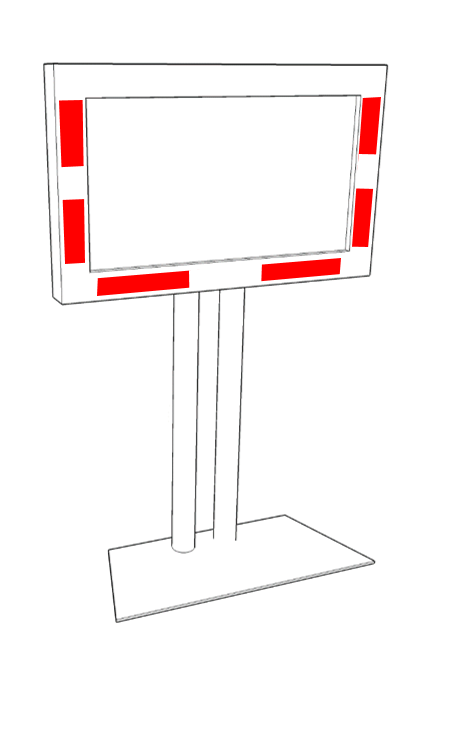
\includegraphics[width=0.4\textwidth]{images/other_proto_capdisp}
\caption{CapDisp sketch - TV on a stand equipped with capacitive sensors hidden below a plastic cover}
\label{fig:other_proto_capdisp}
\end{figure}

CapDisp is a presentation display augmented with capacitive sensors to enable touch-free control of several applications. It was created as a prototype for Hessen IT GmbH in 2010. The system is comprised of six Cypress CY3271 capacitive sensors that are powered via USB and interfaced to a Mini-PC that is attached behind a 42" display on a presentation stand, as shown in a sketch in Figure \ref{fig:other_proto_capdisp}. The display is set in an additional case that hides the six electrodes that are made of copper foil. As shown in Figure \ref{fig:other_proto_capdisp}, they are placed on the bottom and right part of the screen, allowing to detect four different swiping gestures, left and right on the bottom of the screen, up and down on the left side of the screen. The gestures can be performed at a distance of up to 20cm in front of the electrodes. Since the primary purpose of this device is showing presentations, some additional dwell gestures were added, that allow jumping to the first or to the last slide by holding the hand in front of a specific sensor for a certain time. Additionally, two other applications were included, a gesture-controlled image viewer and a video player.

\begin{figure}[ht]
\centering
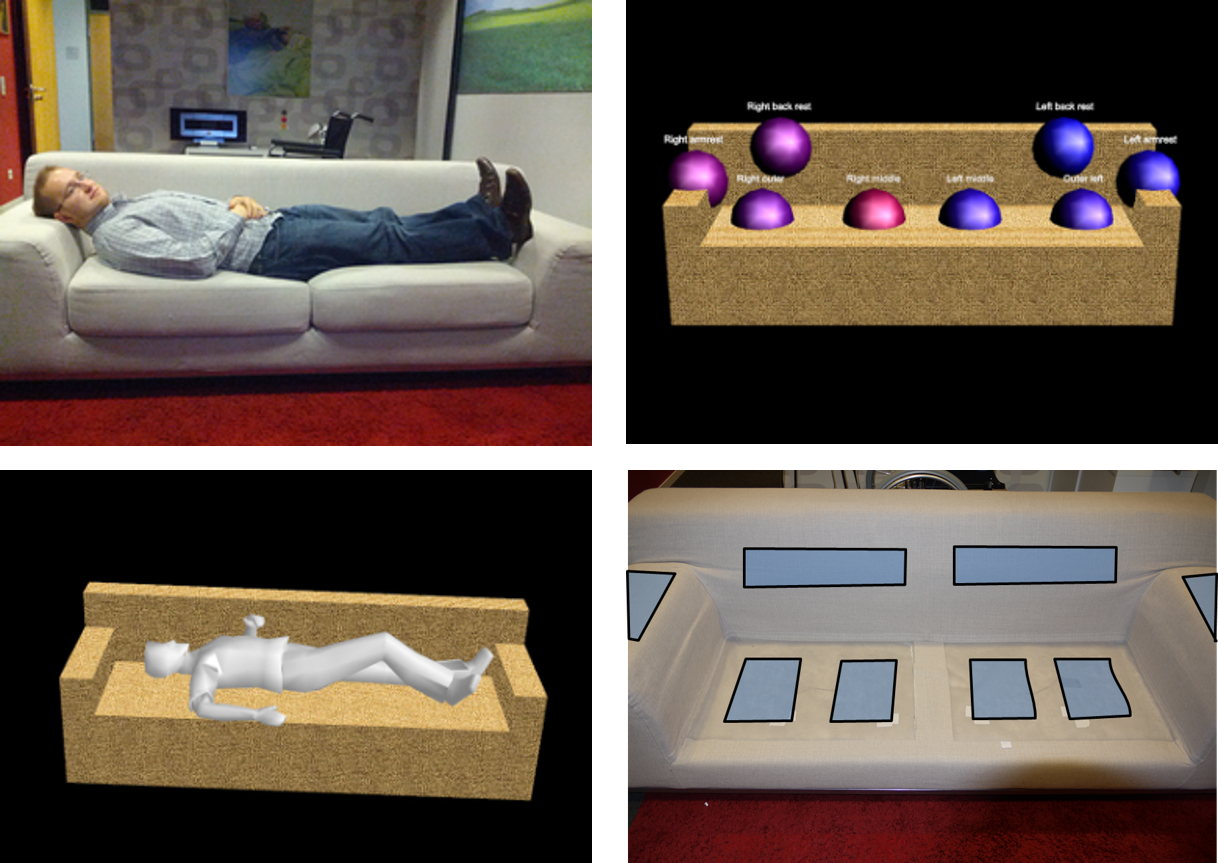
\includegraphics[width=0.8\textwidth]{images/other_proto_smartcouch}
\caption{\emph{Top left}Person lying on the couch. \emph{Top right}Resulting sensor value visualization. \emph{Bottom left}Rendering of recongized posture. \emph{Bottom right}Position of electrodes within the couch.}
\label{fig:other_proto_smartcouch}
\end{figure}

The smart couch was created by then-student Tobias Grosse-Puppendahl in scope of a practical course in 2010/11, supervised by Alexander Marinc and me. The results were later published at the AmI 2011 conference \cite{Couch2011}. Using an array of eight capacitive proximity sensors that are unobtrusively placed inside a couch it is possible to determine the posture of one or more persons that are currently occupying the system. The sensor readings are calibrated and normalized and fed into the WEKA machine learning framework for classification. Three different classifiers have been tested, decision trees, Na\"{i}ve Bayes and RBF networks, whereas the latter provided the best results. The system was evaluated with 18 users and 8 resulting postures (6 with one person, 2 with two persons), such as sitting left or right, or lying in a specific direction. The resulting measurements was distinguished in a training set from 9 persons and a test set from 9 persons. The resulting precision was 97.5\%, the recall 97.2\%. The system is still working as a demonstrator in our living lab, implicitly controlling different networked systems based on the detected postures, e.g. activating ambient lighting as soon as the person is lying down.

\begin{figure}[ht]
\centering
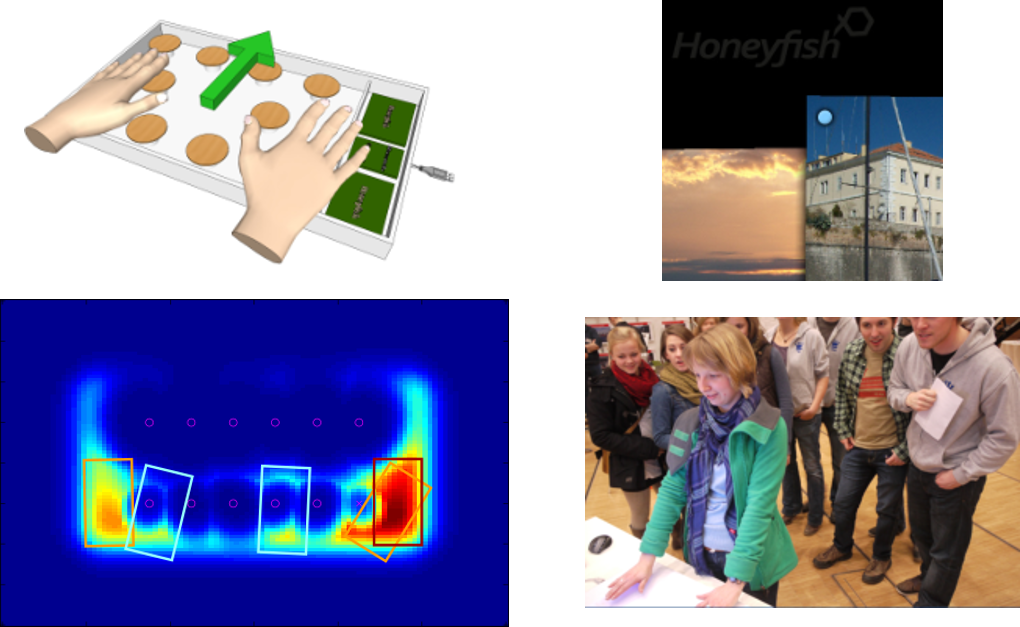
\includegraphics[width=0.8\textwidth]{images/other_proto_honeyfish}
\caption{\emph{Top left} Rendering of Honeyfish device and hands. \emph{Top right} Image of developed GUI and pointer. \emph{Bottom left} Swiss cheese algorithm predicting objects in interaction space. \emph{Bottom right} Evaluation of Honeyfish at a student fair.}
\label{fig:other_proto_honeyfish}
\end{figure}

Honeyfish is a gesture interaction device based on capacitive proximity sensors operated in shunt mode. It was created by Tobias Grosse-Puppendahl in scope of his Master's thesis that I supervised in 2012. It led to two different publications focusing on the provided contributions in multiplexing and object detection \cite{grosse2012honey}\cite{grosse2013swiss}. The system is using eight different transmitters and two receivers, leading to a set of 16 virtual sensors that are set in the middle of each receiver-transmitter combination. As shown in Figure \ref{fig:other_proto_honeyfish} on the top left, the receivers are in the center and the transmitters are placed on the outside. Using a frequency division multiplex it is possible to generate 50 samples from each virtual sensor. The system is using a method of object tracking that extends on a proposal by Smith, dubbed Swiss-cheese, which is based on the premise that each sensor not recognizing an object or a distant object is cutting a (ellipsoid) hole in the object presence probability space, thus leading to a probability distribution visually resembling a Swiss cheese \cite{Smith1996a}. The remaining probability space can be analyzed to fit hand shaped objects, thus enabling gesture detection. A particle filter is used to track the position of the hands. The system is able to track multiple hands and was used to control applications ranging from an image viewer, the GNU TuxRacer game to a remote-controlled vehicle.
\begin{figure}[ht]
\centering
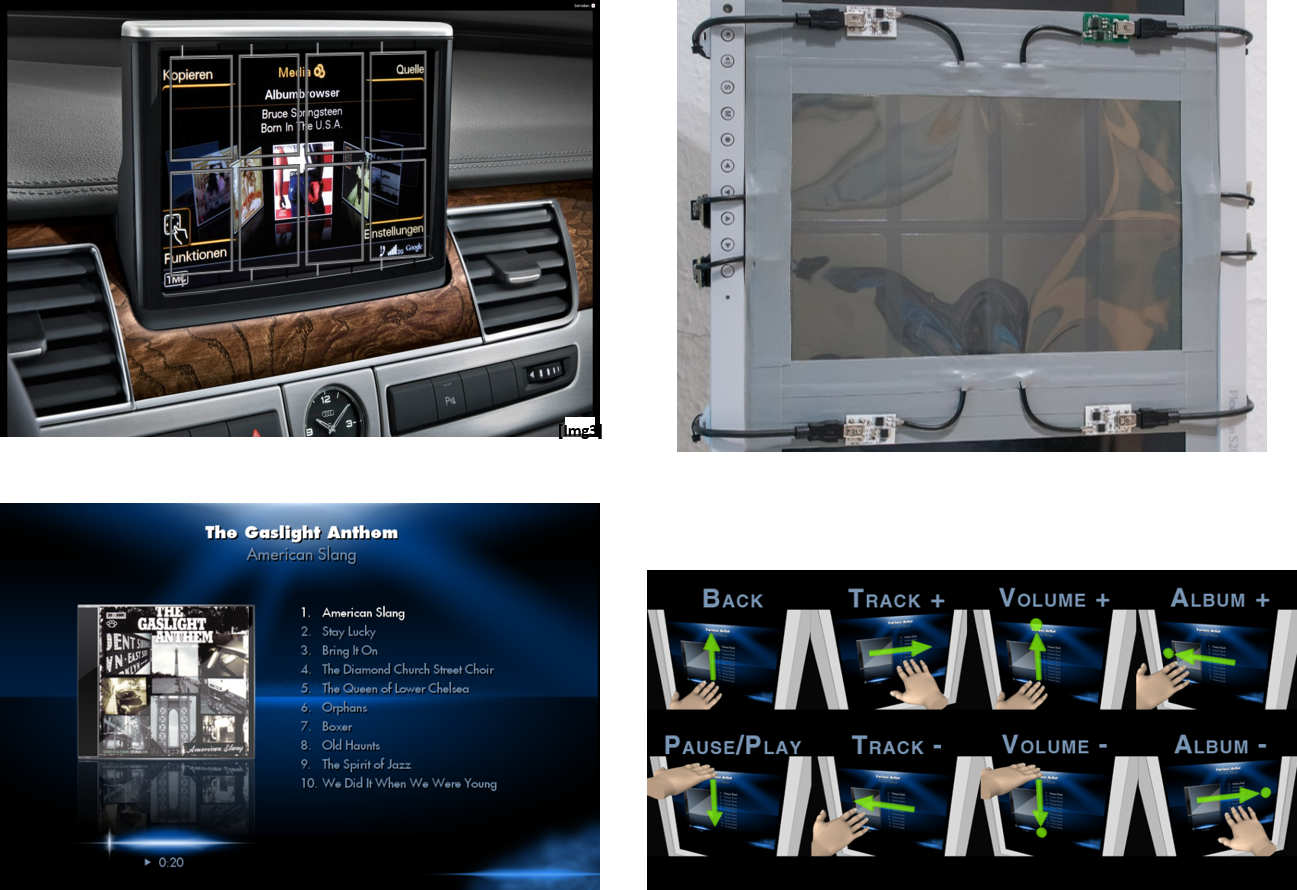
\includegraphics[width=0.8\textwidth]{images/other_proto_gestdisp}
\caption{\emph{Top left} Concept image of GestDisp in a car with outlined electrodes. \emph{Top right} GestDisp prototype installed in front of a monitor. \emph{Bottom left} Screenshot of demonstration application music player. \emph{Bottom right} Association of gestures to functions in the demonstration application.}
\label{fig:other_proto_gestdisp}
\end{figure}

GestDisp is the final prototype discussed in this work. It was created by Yannick Berghöfer in 2013 as part of his Master's thesis that was supervised by me and Tobias Grosse-Puppendahl. The basic idea is to enable gestures performed in front of a screen by applying capacitive proximity sensors on the screen surface. Consequently a different type of electrode material has to be used, that combines conductivity and transparency. Different materials have been evaluated, including ITO (indium-tin oxide) and PEDOT:PSS (a conductive polymer) in order to find a suitable electrode candidate. ITO was chosen and attached to the screen including shielding electrodes, reducing the effect of the electric components used to create this display. Nonetheless, the complex and highly disturbing environment drastically limits the distance in which gestures may be performed. The gestures are recognized using a Hidden-Markov-Model classifier that was trained by the developers.  Using this, it was possible to distinguish swipe gestures in four directions, selection gestures as indicated by dwelling at a certain position and combined swipe-and-hold gestures, whereas the hand is resting in the interaction area after performing a swipe, e.g. used for continuous scrolling or increasing the volume. The gesture recognition includes a specific garbage-gesture that allows to distinguish arbitrary movements in the interaction area from deliberate gestures and has to be trained separately. This approach allows a precision and recall of about 95\% on a collected training set. A demonstration application was created that mimics a multimedia system in a car, allowing to control different radio stations or select music of choice.  
